\documentclass[12pt]{article}
\usepackage{../eplcrypto}
\usepackage{geometry} % see geometry.pdf on how to lay out the page. There's lots.
\geometry{a4paper} % or letter or a5paper or ... etc
% \geometry{landscape} % rotated page geometry
\usepackage[parfill]{parskip}
% See the ``Article customise'' template for come common customisations
\usepackage{amsmath}
\usepackage{graphicx}
\usepackage{amssymb}
\usepackage{algorithmic}
\usepackage{algorithm}
\usepackage{tikz}

\usetikzlibrary{calc,positioning}



\title{Slides09}

%%% BEGIN DOCUMENT
\begin{document}

\maketitle
\tableofcontents
\newpage


\section{The RSA signature}
\subsection{The RSA problem}
\subsubsection{Experiment: $\RSAinv$}
\begin{itemize}
	\item $\langle (N,e),(N,d)\rangle \leftarrow \Gen(1^n)$
	\item $y\leftarrow \ZZ_N^*$
	\item $x \leftarrow \A(N,e,y)$
	\item Define $\RSAinv(n) \define \iff x^e = y \bmod{N}$
\end{itemize}
Assumption:
\begin{itemize}
	\item $\forall$ PPT $\A$, $\exists$ negl. $\negl$ s.t.:
	\begin{equation*}
		Pr[\RSAinv(n)=1] \le \negl(n)
	\end{equation*}
	\item The RSA problem is believed to be hard
	\item Not known to be equivalent to factoring
	\item Best choice for N: Product of two large prime factors
\end{itemize}

\subsection{Building a signature scheme with RSA}
\subsubsection{Simple proposal}
\begin{itemize}
	\item $\Gen(1^n)\define \langle (N,e), (N,d)\rangle $ with $|p|=|p|=n$
	\item $\Sign_{(N,d)}(m) \define [m^d \bmod{N}]$
	\item $\Vrfy_{(N,e)}(m,\sigma) \define [\sigma^e =^? m \bmod{N}]$
\end{itemize}
This simple proposal works, but it is not secure:
\begin{itemize}
	\item No-message attack
	\begin{itemize}
		\item Take $\sigma$ at random
		\item Compute $m \define \sigma^e \bmod{N}$
		\item $(m,\sigma)$ is a forgery
	\end{itemize}
	\item Signature combination
	\begin{itemize}
		\item Suppose $\A$ wants to forge a signature on $m$
		\item $\A$ chooses $m_1$ at random and obtains signature $\sigma_1$
		\item $\A$ computes $m_2 \define m/m_1 \bmod{N}$ and obtains signature $\sigma_2$
		\item Now $\sigma \define \sigma_1 \cdot \sigma_2 \bmod{N}$ is a valid signature on $m$
	\end{itemize}	
\end{itemize}

\subsubsection{Hashed RSA}
Hash the message before applying RSA:
\begin{equation*}
	\sigma(m) \define H(m)^d \bmod{N}
\end{equation*}
Verification is simple:
\begin{equation*}
	\sigma^e =^? H(m) \bmod{N}
\end{equation*}
$H$ must be collision resistant, otherwise one could forge a signature for $m$ from the signature of $m'$ s.t. $H(m)=H(m')$.\\
This construction avoids the attacks that simple scheme suffered in the previous subsection.
\begin{itemize}
	\item No-message attack
	\begin{itemize}
		\item $\A$ would need to find $m$ s.t. $H(m) = \sigma^e \bmod{N}$. This is difficult if $H$ is pre-image resistant.
	\end{itemize}
	\item Signature combination
	\begin{itemize}
		\item $\A$ would need to find $m,m_1,m_2$ s.t.\\
		$H(m) = H(m_1)\cdot H(m_1)\bmod{N} $ which seems difficult for traditional hash functions.
	\end{itemize}	
\end{itemize}
Can we prove that this works $=>$ No. There is no expected propery of $H$ for which hashed RSA signatures can be proven secure in the sense of our definition for hash functions.
\newpage


\section{RSA-FDH}
Define \textbf{RSA-FDH} scheme $\Pi$ as follows.
\begin{itemize}
	\item $\Gen$:  $\langle (N,e,d)\rangle \leftarrow RSA(1^n)$
	\item $\Sign$: On input $(N,d)$ and $m\in \bset^*$, output\\
	$\sigma \define H(m)^d \bmod{N}$
	\item $\Vrfy$ On input $(N,e),m \in \bset^*$ and $\sigma$, output 1 iff\\  $[\sigma^e =^? m \bmod{N}]$
\end{itemize}
\textbf{Theorem:} If the RSA problem is hard, then $\Pi$ is EUF-CMA in the ROM


\section{Encrypting with RSA}
RSA can also be used as a public key encryption scheme (with some addition of randomness). 
\subsection{Padded RSA}
\begin{itemize}
	\item $|m| \in \bset^{\frac{|N|}{2}-2}$ and $r\leftarrow \bset^{|N|-|m|-1}$\\
	$\Enc_{N,e}(m) \define (r||m)^e \bmod{N}$
	\item $\Dec_{N,d}(c) \define c^d \bmod{N}$
\end{itemize}
This is believed to be CPA-secure if the RSA problem is hard.

\section{Certificates and PKI}
The key notion here is a digital certificate, which is simply a signature binding an entity to some public key.
Principle:
\begin{itemize}
	\item Bob generates a key pair $pk,sk$
	\item Bob meets Charlie and convinces him that he is Bob and that $pk$ is his public key
	\item Charlie gives $\cert_{C\rightarrow B}$
	\item Bob can now use $\cert_{C\rightarrow B}$ to introduce himself to anyone who knows Charlie
\end{itemize}
$\cert_{C\rightarrow B}$ is called certificate for Bob's key issued by Charlie: $\Sign_{sk_C}(\text{Bob's key is }pk_B )$
\newpage
Alice must be convinced:
\begin{itemize}
	\item That Charlie's key is $pk_C$
	\item That Charlie is honest
	\item That Charlie does check Bob's identity before issuing $\cert_{C\rightarrow B}$
\end{itemize}
Alice considers Charlie as a \emph{certification authority (CA)}

The certification relationship can be chained:
\begin{itemize}
	\item Bob provides Alice with $pk_B$, $\cert_{C\rightarrow B}$, $\cert_{D\rightarrow C}$, $\cert_{E\rightarrow D}$
	\item If Alice:
	\begin{itemize}
		\item Has a copy of $pk_E$, and knows it is authentic
		\item And knows that C,D,E are good CAs
	\end{itemize}
	Then she can conclude that Bob's public key is $pk_B$
\end{itemize}


\subsection{Hierarchic PKI}
A CA often develops an internal hierarchy:
\begin{itemize}
	\item High-level (super-protected) root CA
	\item Mid-level CAs, certified by higher levels
\end{itemize}

Root CA's key must be transmitted in a secure way
\begin{itemize}
	\item Hand-to-hand given when entering a company
	\item Embedded in web browser
	\item Embedded in operating system
\end{itemize}



\subsection{Flat PKI}
I trust someone's key:
\begin{itemize}
	\item Because I met him personally
	\item Or because I trust the key of someone who trusts him
	\item A recursive relationship
\end{itemize}
Trust level can be associated to each contact (possible to use combined trust)

First-hand certificates must be distributed in a secure way.
\begin{itemize}
	\item Face-to-face meeting (key signing parties)
	\item Read over the phone (key fingerprint)
\end{itemize}

Typical example: PGP



\section{Signatures from the Discrete-Logarithm Problem}
\subsection{Identification Schemes}
An identification scheme is an interactive protocol that allows one party to prove its identity (to authenticate itself) to another. Here, we are interested in the public-key setting where the prover and verifier do not share any secret information (such as a password) in advance, instead the verifier only knows the public key of the prover.


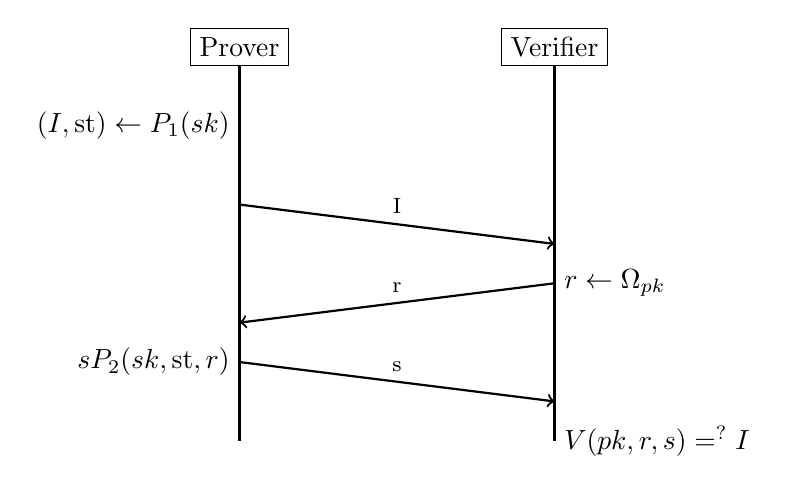
\begin{tikzpicture}
  % Alice
  \node[draw] (Prover) at (-2,0) {Prover}; 
  \draw[thick] (Prover) -- ++(0, -5);
  % Calculations of Alice
  \node[draw=none,fill=none,anchor=east] (asecret) at ($(Prover) + (0,-1)$) {$(I,\text{st}) \leftarrow P_1(sk)$};
  \node[draw=none,fill=none,anchor=east] (asecret) at ($(Prover) + (0,-4)$) {$s \define P_2(sk,\text{st},r)$};
  % Bob
  \node[draw] (Verifier) at (2,0) {Verifier}; 
  \draw[thick] (Verifier) -- ++(0, -5);
   
  % Calculations of Bob
  \node[draw=none,fill=none,anchor=west] (Bpublic) at ($(Verifier) + (0,-3)$) {$r \leftarrow {\Omega_{pk}}$};
  \node[draw=none,fill=none,anchor=west] (Bpublic) at ($(Verifier) + (0,-5)$) {$V(pk, r, s)=^?I$};
   
  % Messages
  \draw[->,thick] ($(Prover)+(0,-2)$) -- ($(Verifier)+(0,-2.5)$) node [pos=0.5,above,font=\footnotesize] {I};
  \draw[->,thick] ($(Verifier)+(0,-3)$) -- ($(Prover)+(0,-3.5)$) node [pos=0.5,above,font=\footnotesize] {r};
  \draw[->,thick] ($(Prover)+(0,-4)$) -- ($(Verifier)+(0,-4.5)$) node [pos=0.5,above,font=\footnotesize] {s};    
\end{tikzpicture}

A general three-round identification protocol of a specific form where the prover is specified by two algorithms $P_1,P_2$ and the verifier's side of the protocol is specified by an algorithm $V$.
\newpage
\subsubsection{Experiment: $\Ident(n)$}
\begin{enumerate}
	\item $\Gen(1^n)$ is run to obtain keys $(pk,sk)$
	\item Adversary $\A$ is given $pk$ and access to an oracle $\mathsf{Trans}_{sk}$ that it can query as often as it likes
	\item At any point during the experiment, $\A$ outputs a message $I$. A uniform challenge $r \in \Omega_{pk}$ is chosen and given to $\A$ who responds with some $s$. ($\A$ may choose to query $\mathsf{Trans}_{sk}$ even after receiving $r$)
	\item The experiment outputs 1 if and only if $V(pk,r,s)=^? I$ 
\end{enumerate}

An identification scheme $\Pi = (\Gen, P_1,P_2,V)$ is secure against a passive attack, or just secure, if $\forall$ PPT $\A$, $\exists$ negl. $\negl$ s.t.:
\begin{equation*}
	Pr[\Ident(n)=1] \le \negl(n)
\end{equation*}

\subsection{From Identification Schemes to Signatures}
The Fiat-Shamir transform provides a way to convert any (interactive) identification scheme into a (non-interactive) signature scheme. The basic idea is for the signer to act as a prover, running the identification protocol by itself.

\subsubsection{Fiat-Shamir transform}
Let $(\Gen_{id}, P_1,P_2,V)$ be an identification scheme, and construct a signature scheme as follows:
\begin{itemize}
	\item $\Gen$: On input $1^n$, simply run $\Gen(1^n)$ to obtain $pk,sk$\\
	The public key $pk$, specifies a set of challenges $\Omega_{pk}$. As part of key generation, a function $H: \bset^* \rightarrow \Omega_{pk} $ is specified (left implicit)
	\item $\Sign$: On input a private key $sk$ and a message $m \in \bset^*$, do:
	\begin{enumerate}
		\item Compute $(I,st) \leftarrow P_1(sk)$
		\item Compute $r \define H(I,m)$
		\item Compute $s\define P_2(sk,st,r)$
	\end{enumerate}
	Output the signature $(r,s)$
	\item $\Vrfy$: On input a public key $pk$, a message $m$, and a signature $(r,s)$, compute $I \define V(pk,r,s)$ and output 1 $\iff H(I,m)=^?r$ 
\end{itemize}

A signature $(r,s)$ is "bound" to a specific message $m$ because $r$ is a function of both $I$ and $m$; changing $m$ thus results in a completely different $r$.


\textbf{Theorem:} Let $\Pi$ be an identification scheme, and let $\Pi'$ be the signature scheme that results by applying the Fiat-Shamir transform to it. If $\Pi$ is secure and $H$ is modelled as a random oracle, then $\Pi'$ is secure. 



\subsection{The Schnorr Identification/Signature Schemes}
The prover runs $(\GG, q, g, y) \leftarrow \G(1^n)$, chooses a uniform $x \in \ZZ_q$ and sets $y \define g^x$, $pk \define \langle \GG,q,g,y \rangle $,  $sk = x$
\subsubsection{Schnorr Identification Scheme}
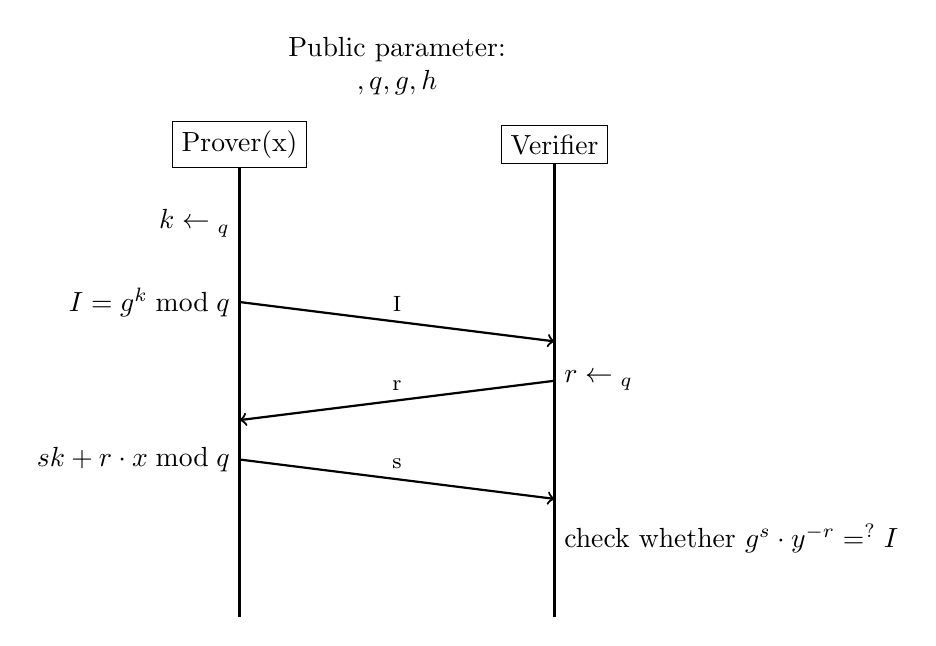
\begin{tikzpicture}
  % Public parameter:
  \node[draw=none,fill=none,align=center] (public) at (0,1) {Public parameter:\\$\GG,q,g,h$};
  % Alice
  \node[draw] (Prover) at (-2,0) {Prover(x)}; 
  \draw[thick] (Prover) -- ++(0, -6);
    
  % Calculations of Alice
  \node[draw=none,fill=none,anchor=east] (asecret) at ($(Prover) + (0,-1)$) {$k \leftarrow {\ZZ_q}$};
  \node[draw=none,fill=none,anchor=east] (Apublic) at ($(Prover) + (0,-2)$) {$I = g^{k} \bmod{q}$};
  \node[draw=none,fill=none,anchor=east] (akey) at ($(Prover) + (0,-4)$) {$s \define k + r \cdot x \bmod{q}$};
    
  % Bob
  \node[draw] (Verifier) at (2,0) {Verifier}; 
  \draw[thick] (Verifier) -- ++(0, -6);
   
  % Calculations of Bob
  \node[draw=none,fill=none,anchor=west] (Bpublic) at ($(Verifier) + (0,-3)$) {$r \leftarrow {\ZZ_q}$};
  \node[draw=none,fill=none,anchor=west] (Bpublic) at ($(Verifier) + (0,-5)$) {check whether $g^s\cdot y^{-r} =^? I$};
   
  % Messages
  \draw[->,thick] ($(Prover)+(0,-2)$) -- ($(Verifier)+(0,-2.5)$) node [pos=0.5,above,font=\footnotesize] {I};
  \draw[->,thick] ($(Verifier)+(0,-3)$) -- ($(Prover)+(0,-3.5)$) node [pos=0.5,above,font=\footnotesize] {r};
  \draw[->,thick] ($(Prover)+(0,-4)$) -- ($(Verifier)+(0,-4.5)$) node [pos=0.5,above,font=\footnotesize] {s};
\end{tikzpicture}

\emph{Passive eavesdropping is no help to the attacker. The reason is that the attacker can simulate the transcripts of honest executions on its own, based on the public key without knowledge of the private key}.\\
Simulation goes as follows:
\begin{enumerate}
	\item Choose uniform and independent $r,s \in \ZZ_q$
	\item Set $I \define g^s\cdot y^{-r}$
\end{enumerate}
Proof idea: We have reduced to an attacker who gets a public key $y$, sends an initial message $I$, is given in response a uniform challenge $r$, and then must send a response $s$ for which $g^s \cdot y^{-r} = I$. If the attacker is able to do this with high probability, then it must be able to compute correct responses $s_1, s_2$ to at least two different challenges $r_1, r_2 \in \ZZ_q$

But then this means that the attacker can now compute the discrete log:
\begin{equation*}
g^{s_1} \cdot y^{-r_1} = I = g^{s_2} \cdot y^{-r_2}
\end{equation*}
\begin{equation*}
g^{s_1 - s_2}  = y^{r_1-r_2}
\end{equation*}
\begin{equation*}
\log_gy = [(s_1-s_2)\cdot (r_1-r_2)^{-1} \bmod{q}]
\end{equation*}
contradicting the assumed hardness of the discrete logarithm.


\subsubsection{Schnorr Signature Scheme}
The Schnorr signature scheme is obtained by applying the Fiat-Shamir transform to the Schnoor identification scheme.

\begin{itemize}
	\item $\Gen$: $(\GG,q,g)\leftarrow \G(1^n)$\\
	$x \leftarrow \ZZ_q$ and set $y\define g^x$\\
	$pk=\langle \GG,q,g, y\rangle$ and $sk=x$
	\item $\Sign$: Input: $(x,m)$\\
	$k \leftarrow \ZZ_q$ and set $I\define g^k$\\
	Compute: $r \define H(I,m)$ and $s\define rx+k \bmod{q}$\\
	Output: $(r,s)$ as signature
	\item $\Vrfy$: Input: $pk,m, (r,s)$\\
	Compute: $I \define g^s\cdot y^{-r}$ and output 1 if $H(I,m)=^?r$
\end{itemize}
















\end{document}